\chapter{Fundamentación Teórica}

El presente capítulo constituye el soporte teórico y técnico sobre el cual se sustenta la propuesta 
de solución para la plataforma Picta. Su propósito es establecer un marco de referencia común que 
permita comprender la complejidad del problema y la validez de la arquitectura propuesta. 

Para ello, la exposición se estructura en cinco momentos fundamentales: primero, se definen los 
conceptos técnicos esenciales que rigen el sistema; segundo, se realiza un estudio comparativo de 
soluciones homólogas en el mercado; tercero, se caracteriza el flujo operativo actual de Picta para 
identificar sus vulnerabilidades; cuarto, se seleccionan las herramientas tecnológicas que integrarán 
la solución; y finalmente, se fundamenta la metodología de desarrollo de software que guiará la 
ejecución del proyecto.

\section{Definiciones y conceptos fundamentales}

Para poder profundizar en el análisis de la infraestructura de Picta, es imprescindible precisar los 
términos técnicos y protocolos que forman la base del sistema objetivo. Esta 
contextualización conceptual garantiza una familiarización con la terminología de 
redes, almacenamiento y procesamiento de video que se empleará de forma recurrente en los capítulos 
posteriores. A continuación, se describen los conceptos clave:

\begin{description}
\sloppy
  \item[Checksum:] El checksum es un valor numérico calculado a partir de una secuencia de datos,
  empleado para verificar la integridad de la información durante su transmisión o almacenamiento.
  Su uso permite detectar alteraciones o corrupciones producidas por fallos de red o de hardware
  \citep{ISO2016}. Es utilizado para validar la integridad
  de cada fragmento de video durante el proceso de subida fragmentada a servicios de almacenamiento de datos.
  Cada trozo recibido debe validarse con su checksum antes de ser almacenado,
  garantizando que no se produjo corrupción de datos durante la transferencia bajo condiciones de
  red inestable.

  \item[Protocolo SSH:] El protocolo SSH (\textit{Secure Shell}) define la arquitectura para el
  inicio de sesión remoto seguro entre computadoras. Provee mecanismos de autenticación robusta y
  protege la integridad y confidencialidad de las comunicaciones mediante cifrado. Constituye el
  sucesor seguro de protocolos como Telnet y métodos de transferencia inseguros como FTP
  \citep{Ylonen2006}.

  \item[Amazon S3:] Amazon Simple Storage Service (Amazon S3) es un servicio de almacenamiento de
  objetos en la nube que ofrece escalabilidad, alta disponibilidad y seguridad para el almacenamiento
  y recuperación de cualquier volumen de datos no estructurados, incluyendo video, imágenes y
  documentos \citep{AWS2023}. Existen sistemas de almacenamiento
  de objetos compatibles con la API de Amazon S3, estos pueden funcionar como servidor de destino para los fragmentos de
  video subidos a una plataforma de streaming. 

  \item[Transcoding:] Proceso de conversión digital entre formatos de codificación de video o audio.
  Comprende la descompresión del contenido original, su transformación ---resolución, tasa de bits,
  códec--- y su recompresión en el formato de destino, con el objetivo de garantizar la
  compatibilidad con distintos dispositivos y condiciones de red \citep{Richardson2003}.
  Esto suele garantizar en muchos sistemas que el procesamiento intensivo de recursos no afecte la 
  interacción del usuario ni obligue a mantener sesiones abiertas innecesariamente.

  \item[Integración \textit{seamless}:] Concepto de arquitectura de software que describe la
  capacidad de un módulo o sistema para integrarse en un entorno existente sin alterar la experiencia
  del usuario ni requerir cambios estructurales en los componentes adyacentes
  \citep{Zhuk2004}. Módulos nuevos, creados con el fin de integrarse con una plataforma en producción sin requerir
  modificaciones significativas en los flujos de autenticación, permisos o gestión de datos existentes, tienen como 
  una buena práctica la integración seamless.

  \item[API:] Una Interfaz de Programación de Aplicaciones (API) define el contrato mediante el
  cual dos componentes de software se comunican. En la arquitectura REST, este contrato se expresa a
  través de recursos, verbos HTTP y representaciones de estado, según los principios establecidos
  en la disertación doctoral de \citet{Fielding2000}. Plataformas como Picta funcionan gracias a estas interfaces
  de programación de aplicaciones, encargándose de manejar la mayor parte de la lógica.

  \item[Frontend y Backend:] En la arquitectura de aplicaciones web, el \textit{frontend} designa
  la capa de presentación con la que interactúa el usuario, mientras que el \textit{backend}
  comprende la lógica de negocio, el acceso a datos y la infraestructura del servidor. Ambas capas
  se comunican mediante interfaces bien definidas \citep{Richards2020}. Muchos sistemas modernos usan estos términos para
  definir una separación clara de responsabilidades entre dos servicios. El frontend reaccionará
  de forma reactiva a los cambios de estado del backend sin necesidad de mantener conexiones persistentes durante el proceso de transcodificación.

  \item[Tarea \textit{ad hoc}:] En gestión de proyectos, una tarea \textit{ad hoc} es una actividad
  no planificada que surge durante la ejecución del proyecto y debe atenderse sin interrumpir el
  flujo principal de trabajo \citep{Wysocki2019}. Durante el proceso de desarrollo usando una metodología ágil, en casi todos los casos con estructura de sprints,
  se permite  la integración controlada de tareas \textit{ad hoc} que surgen de las validaciones con el
  cliente. Estas tareas se incorporan al \textit{Product Backlog} y se priorizan en función de su
  impacto en el objetivo del sprint, sin comprometer la entrega del incremento funcional al cierre de
  la iteración.

  \item[World Wide Web:] Sistema de información distribuida que opera sobre Internet mediante el
  protocolo HTTP, permitiendo la transmisión de documentos de hipertexto e hipermedia. Fue
  concebido originalmente por Tim Berners-Lee en el CERN en 1989
  \citep{BernersLee1992}.

  \item[Framework:] Estructura reutilizable de software que provee un conjunto de abstracciones,
  bibliotecas y convenciones sobre las cuales los desarrolladores construyen aplicaciones. Define
  el esqueleto de la aplicación e invierte el control respecto al código del programador
  \citep{Sommerville2015}.

  \item[SDK:] Un kit de desarrollo de software (\textit{Software Development Kit}) agrupa las
  bibliotecas, herramientas, documentación y ejemplos necesarios para que los desarrolladores
  interactúen programáticamente con una plataforma o servicio determinado
  \citep{Messerschmitt2003}. Un SDK pudiese facilitar operaciones como la creación de buckets, 
  la subida de archivos fragmentados, la validación de checksums y la gestión de metadatos de objetos 
  que se deseen guardar, encapsulando la complejidad de un protocolo y permitiendo que el código del backend 
  se mantenga enfocado en la lógica de negocio.
\end{description}

\section{Sistemas homólogos}

Como parte de la investigación para el desarrollo de la aplicación se realizó un estudio de sistemas
con características similares a las deseadas con el propósito de encontrar una opción que se ajuste a
los requisitos de la tarea o, alternativamente, utilizar el conocimiento obtenido durante el proceso
de investigación en el desarrollo de una solución especializada. 

\begin{description}
\sloppy
  \item[Rsync:] Es una aplicación de línea de comandos que permite la rápida transferencia de
  archivos entre computadoras. Copia las diferencias entre los archivos por lo que en caso de error
  en la transferencia es siempre posible reintentarla con una pérdida mínima de progreso. RSync
  identifica estas diferencias dividiendo los archivos en bloques, generando un checksum para cada
  uno de estos y comparando el resultado. También tiene una función de compresión lo que reduce la
  carga de la red y permite una transferencia más rápida. Finalmente, las transferencias se realizan
  a través del protocolo SSH ofreciendo un alto nivel de seguridad.

  \item[MinIO Client:] MinIO es un sistema de almacenamiento de objetos de alto rendimiento liberado
  bajo la licencia GNU Affero General Public License v3.0. Su API es compatible con el servicio
  Amazon S3 \citep{Gadban2021}. Es capaz de trabajar con información no estructurada como fotos o
  vídeos. MinIO tiene tres componentes: MinIO Server, MinIO Client y MinIO Client SDK. MinIO Client
  es una aplicación de línea de comandos que proporciona una alternativa moderna a comandos UNIX
  como \texttt{ls}, \texttt{cat}, \texttt{cp}, \texttt{mirror} y \texttt{diff}. Soporta sistemas de
  archivos y servicios de almacenamiento en la nube compatibles con Amazon S3
  \citep{Grandhe2026}.

  \item[Filezilla:] Es una aplicación de código abierto liberada bajo la licencia GNU GPL que permite
  interactuar con servidores FTP. Está dividida en Filezilla Client y Filezilla Server, ambos con
  soporte para FTP y FTPS, mientras que el cliente soporta adicionalmente SFTP.
\end{description}

\begin{longtable}[c]{|>{\centering\arraybackslash}p{5cm}|>{\centering\arraybackslash}p{2cm}|>{\centering\arraybackslash}p{2.5cm}|>{\centering\arraybackslash}p{2cm}|}
\caption{Comparación de aplicaciones analizadas}
\label{tb:homologos}\\

\hline
\textbf{Característica} & \textbf{Rsync} & \textbf{MinIO Client} & \textbf{Filezilla} \\
\hline
\endfirsthead

\caption[]{Continuación de la página anterior} \\
\hline
\textbf{Característica} & \textbf{Rsync} & \textbf{MinIO Client} & \textbf{Filezilla} \\
\hline
\endhead

\multicolumn{4}{r}{{Continúa en la próxima página}} \\
\endfoot

\hline
\endlastfoot

Interfaz Gráfica            & No & Sí & Sí \\ \hline
Resistencia a Errores       & Sí & No & No \\ \hline
Filtro de Contenido         & No & No & No \\ \hline
Capacidad de autenticación  & Sí & Sí & Sí \\ \hline

\end{longtable}

Como se aprecia en la Tabla~\ref{tb:homologos}, aunque existen herramientas consolidadas para la
transferencia y gestión de archivos, ninguna ofrece una solución integral que se alinee
completamente con las particularidades del ecosistema de Picta. Herramientas como Rsync destacan
por su robustez y resistencia a fallos de red, pero carecen de una interfaz gráfica orientada a
usuarios no técnicos. Por su parte, opciones como MinIO Client o Filezilla, si bien facilitan la
autenticación y el manejo de objetos, operan como aplicaciones independientes o de línea de
comandos. Esto imposibilita una integración \textit{seamless} dentro del flujo web de la plataforma.

Por consiguiente, el estudio de estos sistemas homólogos permite concluir que la adopción de una
herramienta prefabricada no es viable para este caso de estudio, ya que obligaría a los creadores
de contenido a abandonar el entorno de Picta para utilizar software de terceros, fragmentando la
experiencia de usuario. No obstante, el análisis de sus fortalezas ---como la división en bloques
de Rsync o la compatibilidad S3 de MinIO--- sienta las bases para desarrollar un módulo propio.

\section{Caracterización del flujo actual}

Actualmente, el proceso de publicación en Picta sigue un flujo monolítico y síncrono donde la subida
del video y su posterior renderizado (procesamiento, transcoding y generación de calidades) ocurren de
manera secuencial dentro de una misma transacción. Este esquema presenta tres limitaciones
estructurales que comprometen tanto la experiencia del usuario como la sostenibilidad técnica del
servicio.

En primer lugar, el proceso consume un ancho de banda y recursos del servidor significativos de forma
continua durante toda la operación, dado que cada etapa ---subida, validación, transcoding y
generación de múltiples calidades--- bloquea los recursos hasta su conclusión antes de ceder el
control a la etapa siguiente. En segundo lugar, el flujo es altamente vulnerable a interrupciones de
red: cualquier interrupción durante la transferencia del archivo obliga a reiniciar el proceso
completo desde el inicio, sin posibilidad de reanudación parcial. En tercer lugar, el sistema no
proporciona retroalimentación en tiempo real al usuario sobre el estado de la publicación, lo que
genera incertidumbre e insatisfacción en los creadores de contenido.

El diagrama de la Figura~\ref{fig:flujo_actual} ilustra esta secuencia, destacando los puntos de
fallo y las ineficiencias del modelo actual.

\begin{figure}[H]
  \centering
  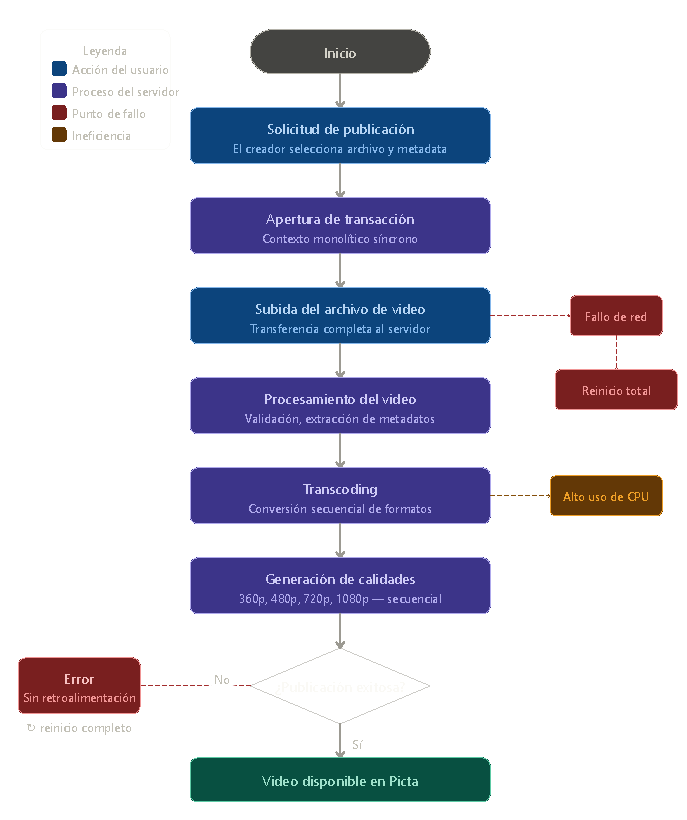
\includegraphics[width=0.9\textwidth]{Images/flujo_actual.pdf}
  \caption{Flujo monolítico y síncrono del proceso de publicación en Picta}
  \label{fig:flujo_actual}
\end{figure}

El conjunto de estas deficiencias genera frustración en los creadores de contenido, ineficiencia en
el uso de los recursos del servidor y limita la escalabilidad horizontal del servicio. Con una
integración transparente en la interfaz existente de Picta, el sistema propuesto será utilizado
tanto por los creadores de contenido como por los administradores de la plataforma, mejorando
radicalmente la resiliencia del servicio ---entendida como la capacidad del sistema de garantizar
la continuidad del proceso ante fallos externos \citep{Avizienis2004}---, la satisfacción del
usuario y la capacidad de la plataforma para crecer de forma sostenible.

\section{Herramientas y Tecnologías}

La selección de las herramientas y tecnologías que integran la solución propuesta responde a un 
criterio de compatibilidad arquitectónica con la plataforma Picta existente, priorizando la cohesión 
del ecosistema tecnológico sobre la adopción de alternativas externas. A continuación, se describen 
el lenguaje de programación, las herramientas de desarrollo y las bibliotecas y \textit{frameworks} 
seleccionados, justificando en cada caso su pertinencia para los objetivos del proyecto.

\subsection{Selección del lenguaje de programación}

La selección del lenguaje para el nuevo módulo está condicionada por la integración con la plataforma
existente. Si bien soluciones alternativas desarrolladas en lenguajes como Golang ofrecerían ventajas
significativas en rendimiento y manejo de concurrencia, la decisión se ve constreñida por la
arquitectura actual del sistema, la cual implementa la API en Python y el frontend en JavaScript,
estableciendo dependencias técnicas que priorizan la cohesión de la plataforma sobre optimizaciones
puntuales.

La evaluación técnica conduce hacia la selección de \textbf{Python} como lenguaje backend. Python
es un lenguaje de programación interpretado, de alto nivel y propósito general, caracterizado por
una sintaxis clara que favorece la legibilidad y reduce el costo de mantenimiento del código.
Cuenta con un amplio ecosistema de bibliotecas para desarrollo web, computación científica y
automatización \citep{Pressman2021}, lo que lo hace especialmente adecuado para la construcción
de módulos de integración como el que se propone.

Paralelamente, para el frontend se mantiene la coherencia arquitectónica mediante la adopción de
\textbf{JavaScript}. Según el estándar ECMAScript, JavaScript es el lenguaje de scripting del lado
del cliente predominante en la Web, y su especificación define el modelo de ejecución, los tipos
de datos y los mecanismos de concurrencia basados en eventos que se utilizarán en el componente
Angular del módulo \citep{Ecma2023}.

\subsection{Herramientas utilizadas}

Las siguientes herramientas fueron empleadas directamente durante el ciclo de desarrollo del módulo,
cubriendo las etapas de codificación, gestión de base de datos, prueba de interfaces y modelado.

\begin{description}
\sloppy
  \item[Visual Studio Code v1.106.2:] Editor de código fuente desarrollado por Microsoft para
  Windows, Linux, macOS y Web. Incluye soporte para depuración, control integrado de Git, resaltado
  de sintaxis, finalización inteligente de código y refactorización. Es software gratuito y de
  código abierto. Fue utilizado como entorno principal de desarrollo del módulo.

  \item[Navicat Premium v17.1.10:] Software de gestión y administración de bases de datos que
  permite conectarse y administrar múltiples motores, incluyendo PostgreSQL, MySQL, MariaDB y
  SQL Server \citep{Sommerville2015}. Se empleó para inspeccionar, consultar y verificar el estado
  de la base de datos de Picta durante el desarrollo e integración del módulo.

  \item[Postman v11.73.3:] Herramienta para el desarrollo, prueba y documentación de APIs. Su
  interfaz gráfica permite construir, enviar y validar solicitudes HTTP de forma sistemática,
  facilitando la verificación de contratos de interfaz \citep{Lutz2013}. Se utilizó para probar
  todos los endpoints de la API desarrollada y documentar el comportamiento del módulo de subida.

  \item[S3 Browser v12.9.9:] Cliente de escritorio para la administración de almacenamiento de
  objetos compatible con el protocolo S3 \citep{AWS2023}. Durante las pruebas, se empleó para
  inspeccionar y verificar la integridad y ubicación de los fragmentos almacenados en el servidor
  MinIO.

  \item[Visual Paradigm v17.0:] Herramienta de modelado visual que implementa el estándar UML 2.0
  \citep{Miles2006}. Se utilizó para la elaboración de los diagramas de casos de uso, clases y
  secuencia del proyecto.
\end{description}

\subsection{Bibliotecas y Frameworks utilizados}

En alineación con los criterios derivados del análisis arquitectónico del sistema vigente y con el
objetivo de garantizar una integración totalmente compatible y sin impactos estructurales, se ha
determinado la adopción de los mismos frameworks actualmente utilizados por la plataforma en sus
componentes principales.

\begin{description}
\sloppy
  \item[Django v3.2.2:] Framework web de alto nivel para Python que implementa el patrón
  Modelo-Vista-Template (MVT) y provee componentes integrados para autenticación, ORM, enrutamiento
  y administración. Fomenta el desarrollo rápido y un diseño limpio bajo el principio
  \textit{Don't Repeat Yourself} (DRY) \citep{Christie2024}.

  \item[Angular v15.2.10:] Framework de desarrollo de aplicaciones web de una sola página (SPA)
  basado en TypeScript, mantenido por Google. Implementa una arquitectura de componentes, inyección
  de dependencias y un sistema de módulos que facilita la escalabilidad del frontend
  \citep{Richards2020}.
\end{description}

Con el fin de garantizar una interacción óptima con MinIO, reducir la complejidad operacional y
estandarizar el flujo de integración, se seleccionaron las siguientes librerías especializadas como
componentes primarios de interoperabilidad.

\begin{description}
\sloppy
  \item[Django Rest Framework v3.12.4:] Conjunto de herramientas para la construcción de APIs web
  sobre Django. Provee serializadores, vistas basadas en clases, autenticación y negociación de
  contenido, simplificando la creación de interfaces RESTful robustas y escalables
  \citep{Christie2024}.

  \item[MinIO Python SDK v7.2.18:] SDK de cliente Python que provee una API de alto nivel para
  interactuar con servidores MinIO y cualquier almacenamiento compatible con el protocolo Amazon S3.
  Gestiona operaciones de carga, descarga, listado y eliminación de objetos \citep{MinIO2024}.
\end{description}

\section{Selección de una metodología de desarrollo}

Una metodología de desarrollo de software es un conjunto de prácticas, técnicas y herramientas
utilizadas por los equipos de desarrollo de software para planificar, diseñar, construir, probar y
entregar software de alta calidad de manera eficiente y efectiva \citep{Pressman2021}.

Las metodologías de desarrollo se dividen actualmente en dos enfoques generales: el tradicional y
el ágil. Las metodologías tradicionales se caracterizan por fases predefinidas con un flujo del
desarrollo unidireccional, pasando de la recolección de requisitos al diseño y del diseño al
desarrollo, luego a las pruebas y el mantenimiento. En aproximaciones clásicas como el modelo de
cascada, cada fase genera artefactos y documentación que han pasado por un extensivo proceso de
revisión \citep{Sommerville2015}. Los métodos tradicionales son mejor utilizados en situaciones en
las que los requisitos están bien definidos. En industrias que cambian rápidamente, como la del
desarrollo de software, las metodologías tradicionales pueden fallar en alcanzar sus objetivos.

Dado que los requisitos del módulo a desarrollar son evolutivos ---determinados por la integración
progresiva con una plataforma en producción--- se descarta el enfoque tradicional y se orienta la
selección hacia las metodologías ágiles. Dentro de este grupo, los marcos de trabajo más relevantes
para proyectos de desarrollo de software de alcance acotado son Scrum, Kanban y Extreme Programming
(XP), cuyas características se comparan en la Tabla~\ref{tb:metodologias_agiles}.

\begin{longtable}[c]{|p{2.3cm}|p{5.5cm}|p{5.3cm}|}
\caption{Comparativa de metodologías ágiles}
\label{tb:metodologias_agiles}\\
\hline
\textbf{Metodología} & \textbf{Ventajas} & \textbf{Desventajas} \\
\hline
\endfirsthead
\caption[]{Continuación de la página anterior} \\
\hline
\textbf{Metodología} & \textbf{Ventajas} & \textbf{Desventajas} \\
\hline
\endhead
\multicolumn{3}{r}{{Continúa en la próxima página}} \\
\endfoot
\hline
\endlastfoot

Scrum &
Iteraciones cortas y planificadas (\textit{sprints}). Roles bien definidos. Revisión continua con
el cliente. Adecuado para equipos pequeños y proyectos de complejidad media-alta
\citep{Schwaber2020}. &
Requiere disponibilidad regular del cliente. Puede generar sobrecarga de reuniones si no se
gestiona. Difícil de escalar sin adaptaciones. \\ \hline

Kanban &
Flujo continuo sin iteraciones fijas. Bajo costo de adopción. Útil para equipos con carga variable
o trabajo de mantenimiento \citep{Pressman2021}. &
Sin estructura de planificación temporal. Dificulta la estimación de plazos. Poco adecuado para
proyectos con entregas definidas y cliente activo. \\ \hline

Extreme Programming (XP) &
Énfasis en calidad técnica: pruebas continuas, integración frecuente, refactorización constante.
Adecuado cuando la calidad del código es prioritaria \citep{Pressman2021}. &
Requiere un equipo de al menos dos desarrolladores para prácticas como la programación en pares.
Alta disciplina técnica exigida desde el inicio. \\ \hline

\end{longtable}

Del análisis comparativo se desprende que \textbf{Kanban} no resulta adecuado para este proyecto,
dado que no provee una estructura de planificación temporal que permita gestionar entregas acordadas
con el tutor y el cliente. \textbf{XP}, por su parte, presupone un equipo mínimo de dos
desarrolladores para aplicar sus prácticas centrales ---como la programación en pares y las pruebas
de aceptación en cliente--- lo que lo hace inviable en el contexto de un desarrollador único. En
consecuencia, se selecciona \textbf{SCRUM} como metodología de desarrollo.

Scrum es un marco de trabajo para el desarrollo ágil de software, cuya guía definitiva fue
publicada por sus cocreadores Ken Schwaber y Jeff Sutherland \citep{Schwaber2020}. Es un proceso
en el que se aplican de manera regular un conjunto de buenas prácticas para trabajar
colaborativamente, en equipo y obtener el mejor resultado posible de proyectos, caracterizado por:

\begin{itemize}
  \item Adoptar una estrategia de desarrollo incremental, en lugar de la planificación y ejecución
  completa del producto.

  \item Basar la calidad del resultado más en el conocimiento tácito de las personas en equipos
  autoorganizados, que en la calidad de los procesos empleados.

  \item Solapar las diferentes fases del desarrollo, en lugar de realizar una tras otra en un ciclo
  secuencial o en cascada.
\end{itemize}

Scrum es un marco de trabajo que resulta fácil de aprender, pero difícil de dominar. La esencia
de \textit{Scrum} es un equipo autoorganizado que aporta valor al cliente en períodos limitados
conocidos como \textit{Sprints} \citep{Sutherland2014}.

\begin{figure}[H]
  \centering
  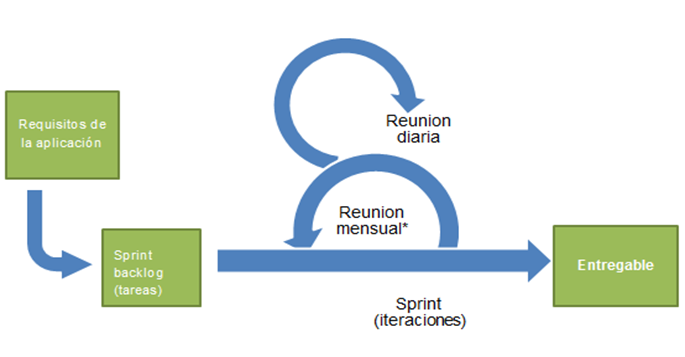
\includegraphics[width=0.9\textwidth]{Images/scrum}
  \caption{Marco de Trabajo SCRUM. Fuente: Adaptado de \citep{AnaDianaMets2013}}
  \label{fig:scrum}
\end{figure}

\subsection{Roles en SCRUM}

La estructura de Scrum se articula en torno a tres roles fundamentales, cada uno con
responsabilidades claramente delimitadas que garantizan el funcionamiento del marco de trabajo
\citep{Schwaber2020}.

El \textbf{Product Owner} es el responsable de maximizar el valor del producto. Representa los
intereses del cliente y de los usuarios finales, gestiona y prioriza el \textit{Product Backlog}
---la lista ordenada de todo lo que el producto podría necesitar--- y toma las decisiones finales
sobre qué se construye y en qué orden. Su efectividad depende directamente de su disponibilidad y
conocimiento del dominio del problema.

El \textbf{Scrum Master} es el garante del proceso \citep{Avizienis2004}. Su función no es la de
un jefe de proyecto tradicional, sino la de un facilitador que protege al equipo de impedimentos
externos, vela por la correcta aplicación del marco Scrum, y promueve la mejora continua a través
de las retrospectivas de sprint. En equipos pequeños, el Scrum Master asume además una función de
\textit{coaching} técnico, orientando las decisiones de diseño y arquitectura cuando el equipo
carece de experiencia suficiente.

El \textbf{Equipo de Desarrollo} está compuesto por los profesionales que ejecutan el trabajo de
construcción del producto. Scrum no prescribe roles internos dentro del equipo ---no hay
distinción formal entre frontend, backend o QA--- y en su lugar promueve la autoorganización: el
equipo decide colectivamente cómo abordar cada ítem del sprint para alcanzar el objetivo acordado
\citep{Cohn2004}.

En el contexto particular de este proyecto, la reducción del equipo a un único integrante implica
la fusión de los roles de \textbf{Scrum Master} y \textbf{Equipo de Desarrollo} en una misma
persona. Esta configuración es viable siempre que el rol de Product Owner permanezca diferenciado
y sea asumido por el cliente \citep{Pierra2022}. En este caso, dicho rol corresponde al
representante de la plataforma Picta, quien valida los incrementos al cierre de cada sprint y
prioriza el backlog en función de las necesidades operativas de la plataforma. El desarrollador
asume el rol de Scrum Master porque es quien posee el conocimiento más profundo de la arquitectura
propuesta, la capacidad para identificar impedimentos técnicos de forma temprana y la
responsabilidad directa de garantizar que cada sprint produzca un incremento funcional e integrable
sobre la plataforma en producción.

La elección de SCRUM para este proyecto se fundamenta en tres factores determinantes que se alinean
con sus fortalezas estructurales. En primer lugar, el equipo de desarrollo está integrado por un
único desarrollador, lo que hace que la ligereza organizativa de Scrum ---frente a metodologías
más pesadas--- sea una ventaja directa. En segundo lugar, el cliente de la plataforma Picta dispone
de alta disponibilidad técnica y conocimiento del dominio, lo que facilita la validación de los
incrementos al cierre de cada sprint. En tercer lugar, la complejidad del proyecto ---integración
de subida fragmentada con arquitectura dirigida por eventos sobre una plataforma en producción---
se ubica dentro del rango de complejidad media-alta que Scrum gestiona con mayor eficacia que un
flujo continuo como Kanban \citep{Schwaber2020}.

\section{Conclusiones Parciales}

El análisis del flujo actual de publicación en Picta evidenció tres limitaciones estructurales ---
consumo continuo de recursos, vulnerabilidad ante interrupciones de red y ausencia de
retroalimentación en tiempo real--- que justifican el desarrollo de una solución especializada. El
estudio de sistemas homólogos confirmó que ninguna herramienta existente satisface los requisitos
de integración \textit{seamless} propios del ecosistema de la plataforma, sentando las bases para
un módulo propio. En este capítulo se definieron además los lenguajes de programación, herramientas,
\textit{frameworks}, librerías y la metodología SCRUM como marco de desarrollo, sustentados en
fuentes primarias y estándares internacionales de la disciplina.